\documentclass[11pt, oneside]{article}   	% use "amsart" instead of "article" for AMSLaTeX format
\usepackage{geometry}                		% See geometry.pdf to learn the layout options. There are lots.
\geometry{letterpaper}                   		% ... or a4paper or a5paper or ... 
%\geometry{landscape}                		% Activate for rotated page geometry
%\usepackage[parfill]{parskip}    		% Activate to begin paragraphs with an empty line rather than an indent
\usepackage{graphicx}				% Use pdf, png, jpg, or eps§ with pdflatex; use eps in DVI mode
								% TeX will automatically convert eps --> pdf in pdflatex		
\usepackage{amssymb}
\usepackage{hyperref}
\usepackage{graphicx}
\graphicspath{{img/}}
%SetFonts

%SetFonts


\title{Learning to Play a Game Using Neural Networks and a Genetic Algorithm}
\author{Kyle Weaver and Rocco Manzo}
%\date{}							% Activate to display a given date or no date

\begin{document}
\maketitle

\begin{abstract}
\end{abstract}

\section{The Dinosaur Game}
%\subsection{}
We chose the Google Chrome dinosaur game to test our genetic algorithm. The game appears when the user presses space (on a keyboard) or taps the screen (on a touch screen) while Chrome does not detect an internet connection. The player controls a dinosaur running across a field populated by obstacles (cacti and pterodactyls). The player makes the dinosaur jump or duck to avoid these obstacles; if the dinosaur runs into an obstacle, the game ends. The goal is to make the dinosaur run as long as possible before colliding with an obstacle. Our reasons for choosing this game were twofold. As part of open-source Chromium project, the game's \href{https://github.com/chromium/chromium/tree/master/components/neterror/resources}{source code} was available for us to modify to suit our needs. The game is also an ideal test subject because its simplicity limits the number of inputs and outputs needed in a neural network.
\begin{figure}[h]
\caption{Screenshot of the Chrome dinosaur game}
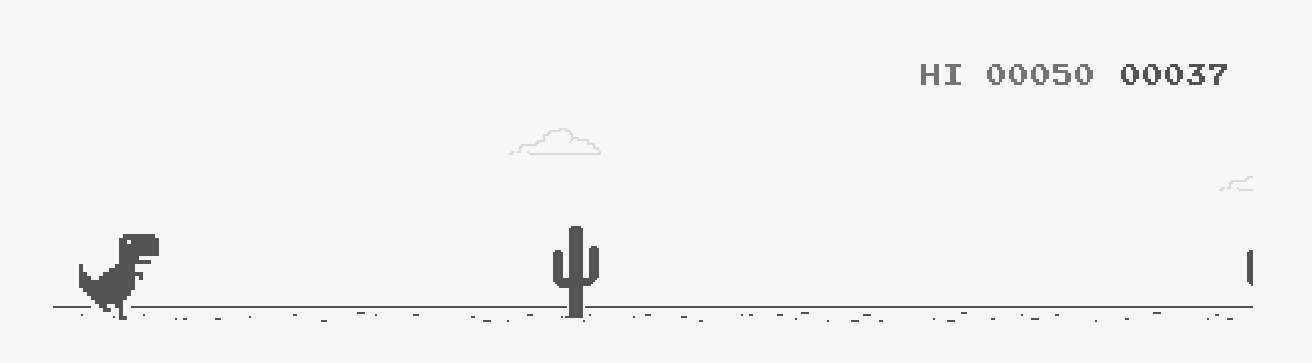
\includegraphics[width=\textwidth]{dino}
\end{figure}

We had to make some adjustments to the game to adapt it to our algorithm. For instance, the original game features a single dinosaur, while we wanted to make a whole generation of dinosaurs run the same course simultaneously. In order to measure the fitness of each individual dinosaur, when one dinosaur collides with an obstacle, we record the distance it ran and stop it from running any further. Instead of ending the game upon the first collision, our modified game keeps running until no dinosaurs remain. Finally, when the game does end, instead of waiting for user input to restart the game, we have the game restart automatically after some set delay.

Our modified game code is found in the file \verb|src/offline.js|.

\end{document}
